%!TEX root = ../thesis.tex

\section{背景}
近年, 機械学習を用いた自律走行に関する研究が盛んにされており, その中でカメラ画像を用いてロボットへ自律走行を行わせる研究もされている. Bojarskiら\cite{bojarski}は\figref{Fig:bojarski_train}に示すシステムで, 人間のドライバーが操作するステアリング角度と前方カメラ画像を用いて模倣学習を行った. また, \figref{Fig:bojarski_test}に示すように, 訓練したネットワークに画像を入力し, 生成される操舵指令を用いて走行を行う手法を提案した.

\vspace{0.5cm}

\begin{figure}[hbtp]
  \centering
 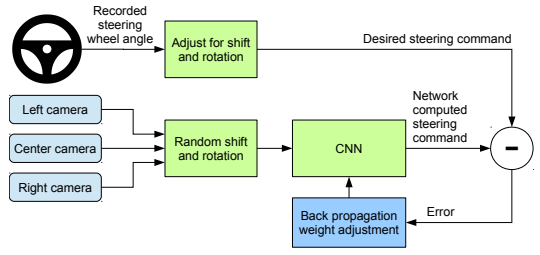
\includegraphics[keepaspectratio, scale=0.9]
      {images/bojarski_train.png}
 \caption{Training the neural network from \cite{bojarski}}
 \label{Fig:bojarski_train}
\end{figure}

\begin{figure}[hbtp]
     \centering
    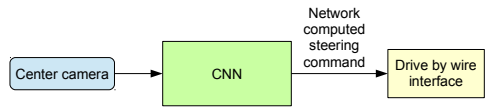
\includegraphics[keepaspectratio, scale=0.6]
         {images/bojarski_test.png}
    \caption{The trained network is used generate steering commands from a single front-facing center camera from \cite{bojarski}}
    \label{Fig:bojarski_test}
\end{figure}

\newpage

本研究室においても, 岡田ら\cite{okada1}はfigに示すようなシステムを用いてfigのように経路追従行動を模倣学習し, カメラ画像に基づいた経路追従行動を獲得した. このシステムでは, LiDAR, オドメトリを入力としたルールベース制御器(後述する”地図を用いたルールベース制御器”)による経路追従行動を前方カメラ画像を用いてend-to-endで模倣学習した. 

\begin{figure}[hbtp]
     \centering
     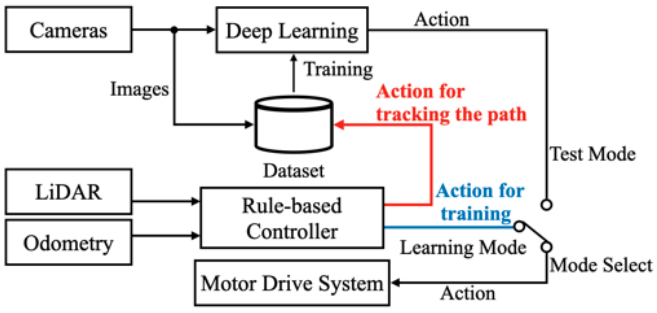
\includegraphics[keepaspectratio, scale=0.5]
          {images/okada_structure.png}
     \caption{The trained network is used generate steering commands from a single front-facing center camera from \cite{okada1}}
     \label{Fig:okada_structure}
\end{figure}

\begin{figure}[hbtp]
     \centering
    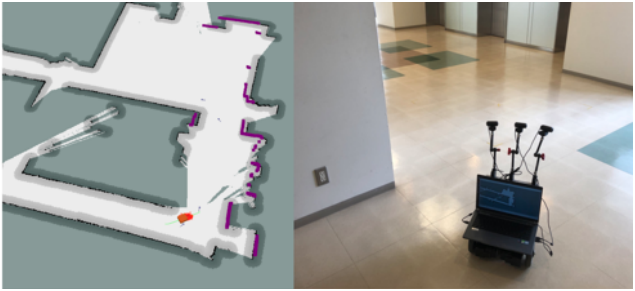
\includegraphics[keepaspectratio, scale=0.5]
         {images/okada_nav.png}
    \caption{Training the neural network from \cite{okada1}}
    \label{Fig:okada_nav}
   \end{figure}

\newpage
